\documentclass[12pt]{beamer}

%%%%%%%%%%%%%%%%%%% Theme

\usetheme{metropolis}

%%%%%%%%%%%%%%%%%%% Packages

\usepackage[french, english]{babel}
\usepackage{packages/sleek-beamer}

%%%%%%%%%%%%%%%%%%% Bibliography

\addbibresource{./resources/bib/references.bib}

%%%%%%%%%%%%%%%%%%% Titlepage

\title{Renewable Energy Production Forecast}
\subtitle{PROJ0016 - Big Data Project}
\author{Yann Claes, Gaspard Lambrechts and François Rozet}
\institute{University of Liège}
\date{\today}
\titlelogo{./resources/pdf/logo.pdf}
\framelogo{./resources/pdf/logo.pdf}

%%%%%%%%%%%%%%%%%%%

\DeclareSIUnit\voltampere{VA}

%%%%%%%%%%%%%%%%%%%

\begin{document}

\maketitle

\section{Photovoltaic production}
\section{Tests of the provincial model}

\begin{frame}{Reminder}
    \begin{itemize}
        \item \alert{Output power} given by
        \begin{equation*}
            P = \eta I A \quad [W]
        \end{equation*}
        with $A = area\_peak * peak\_power$
        \item Use production measurements from Elia to \alert{fit} these 4 parameters
        \item \alert{Predict} production using a normal distribution and irradiance forecasts
    \end{itemize}
\end{frame}

\begin{frame}{Testing procedure}
    \begin{itemize}
        \item Fit the parameters on collected measures for the \alert{past 7 days}
        \item Use this posterior model to make predictions for the \alert{current} day
        \item \alert{Repeat} for each day of 2019
    \end{itemize}
\end{frame}

\begin{frame}{Baseline models}
    We constructed 2 very simple baseline models:
    \begin{itemize}
        \item Predict for day $D + 1$ the \alert{production} measured by Elia for day \alert{$D$}
        \item Predict for day $D + 1$ the \alert{average} production measured by Elia over the last 7 days
    \end{itemize}
\end{frame}

\begin{frame}{Error metrics}
    To \alert{assess} the posterior and baseline models, we use the MSE and RMSE.
    
    We also compute these metrics for our prior model and for the predictions made by \alert{Elia}.
    
    Eventually, we \alert{average} these measures over all conducted tests.
\end{frame}

\begin{frame}{Results}
    \begin{table}
	\centering
    \begin{tabular}{l|c|c}
                        & MSE      & RMSE   \\ \hline
        Prior model     & 682.451  & 23.617 \\ \hline
        \alert{Posterior model} & 469.842  & 19.398 \\ \hline
        Baseline 1      & 2361.555 & 40.390 \\ \hline
        Baseline 2      & 2003.102 & 39.617 \\ \hline
        \alert{Elia's forecast} & 423.539  & 17.891
    \end{tabular}
    \noskipcaption{Mean of the MSE and RMSE (MW) for 2019.}
    \label{tab:pv_metrics_meas}
\end{table}
\end{frame}

\begin{frame}{Conclusions}
    \begin{itemize}
        \item The \alert{posterior model} seems to perform \alert{better} than the baseline and prior models
        \item Elia's forecast is better but we reach, on average, \alert{reasonable} results
        \item These results are obtained using \alert{irradiance measurements}, not irradiance forecasts
    \end{itemize}
\end{frame}

\section{Introducing forecasts}

\begin{frame}{Collecting forecast measures}
    \alert{Forecast measures} have been collected from \alert{April 2\up{nd}} and cover up to 7 days from the current day
\end{frame}

\begin{frame}{Introducing forecasts in the model}
    \begin{itemize}
        \item \alert{Similar} comparison procedure
        \item \alert{No access} to past irradiance forecasts
        \item Fit on \alert{past} irradiance measurements
        \item Predict using irradiance \alert{forecasts}
    \end{itemize}
\end{frame}

\begin{frame}{Testing the model on forecasts}
    A first test has been conducted for a period of \alert{10 days}, starting the predictions from \alert{April 3\up{rd}}.
\end{frame}

\begin{frame}{Results}
    \begin{table}
	\centering
    \begin{tabular}{l|c|c}
                        & MSE      & RMSE   \\ \hline
        Prior model     & 2797.307  & 50.281 \\ \hline
        Posterior model & 1385.751  & 32.594 \\ \hline
        Baseline 1      & 1294.487 & 24.136 \\ \hline
        Baseline 2      & 1039.525 & 27.152 \\ \hline
        Elia's forecast & 292.916  & 15.219
    \end{tabular}
    \noskipcaption{Mean of the MSE and RMSE (MW) for 10 days.}
    \label{tab:pv_metrics_for}
\end{table}
\end{frame}

\begin{frame}{Conclusions}
    \begin{itemize}
        \item \alert{Posterior} model performs \alert{better} than our prior model
        \item \alert{Baseline} models both \alert{outperform} our posterior model
    \end{itemize}
\end{frame}

\begin{frame}{Conclusions}
    \begin{figure}
    \centering
    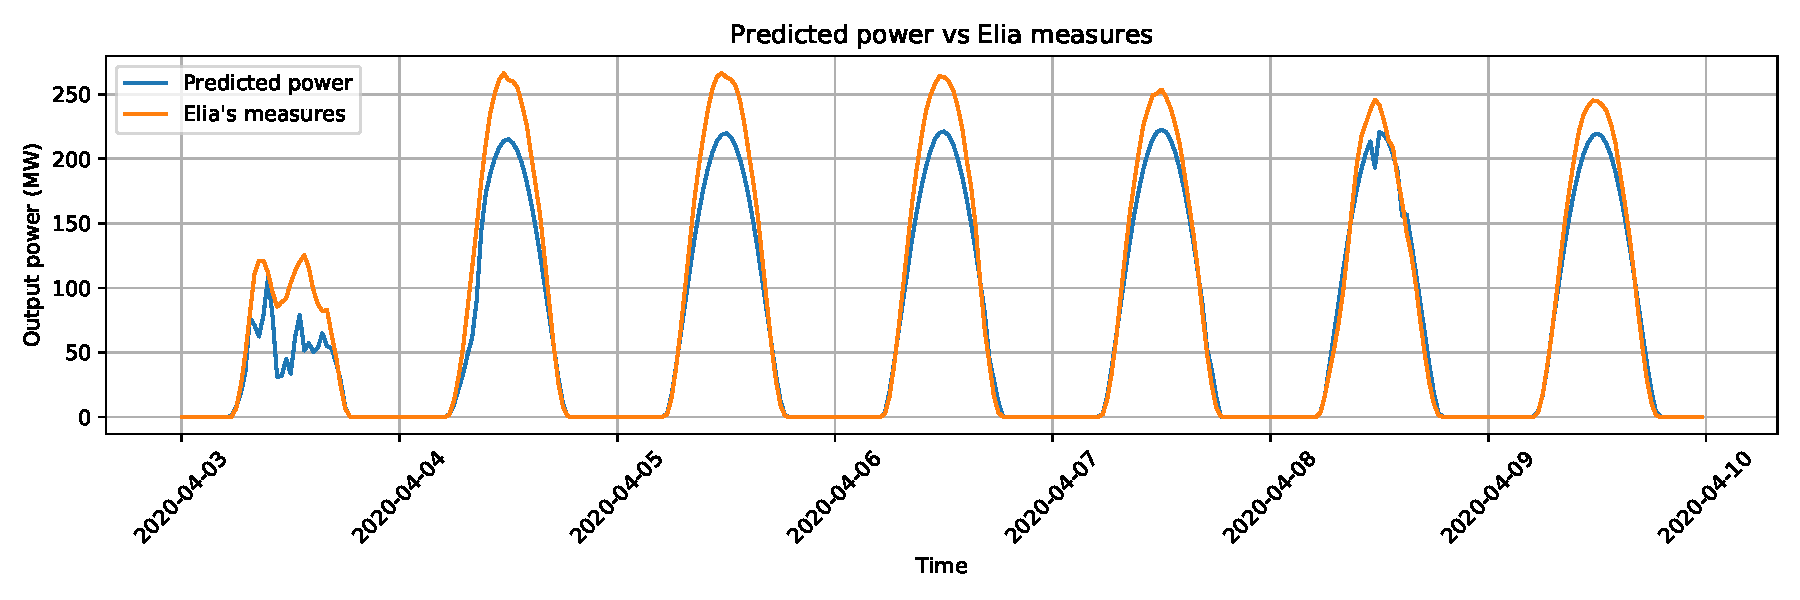
\includegraphics[width=\textwidth]{resources/pdf/province_naive_03-04-2020.pdf}
    \noskipcaption{Comparison between Elia's measurements and the prior model (using irradiance measurements).}
    \label{fig:prior_model}
\end{figure}
\end{frame}

\begin{frame}{Conclusions}
    \begin{itemize}
        \item \alert{Measurements} made by Elia over this period are all very \alert{similar}
        \item Baseline models \alert{use} past data \emph{as is}
        \item \alert{Forecasts} are sometimes \alert{unreliable}
    \end{itemize}
\end{frame}

\begin{frame}{Conclusions}
    \begin{figure}[H]
    \centering
    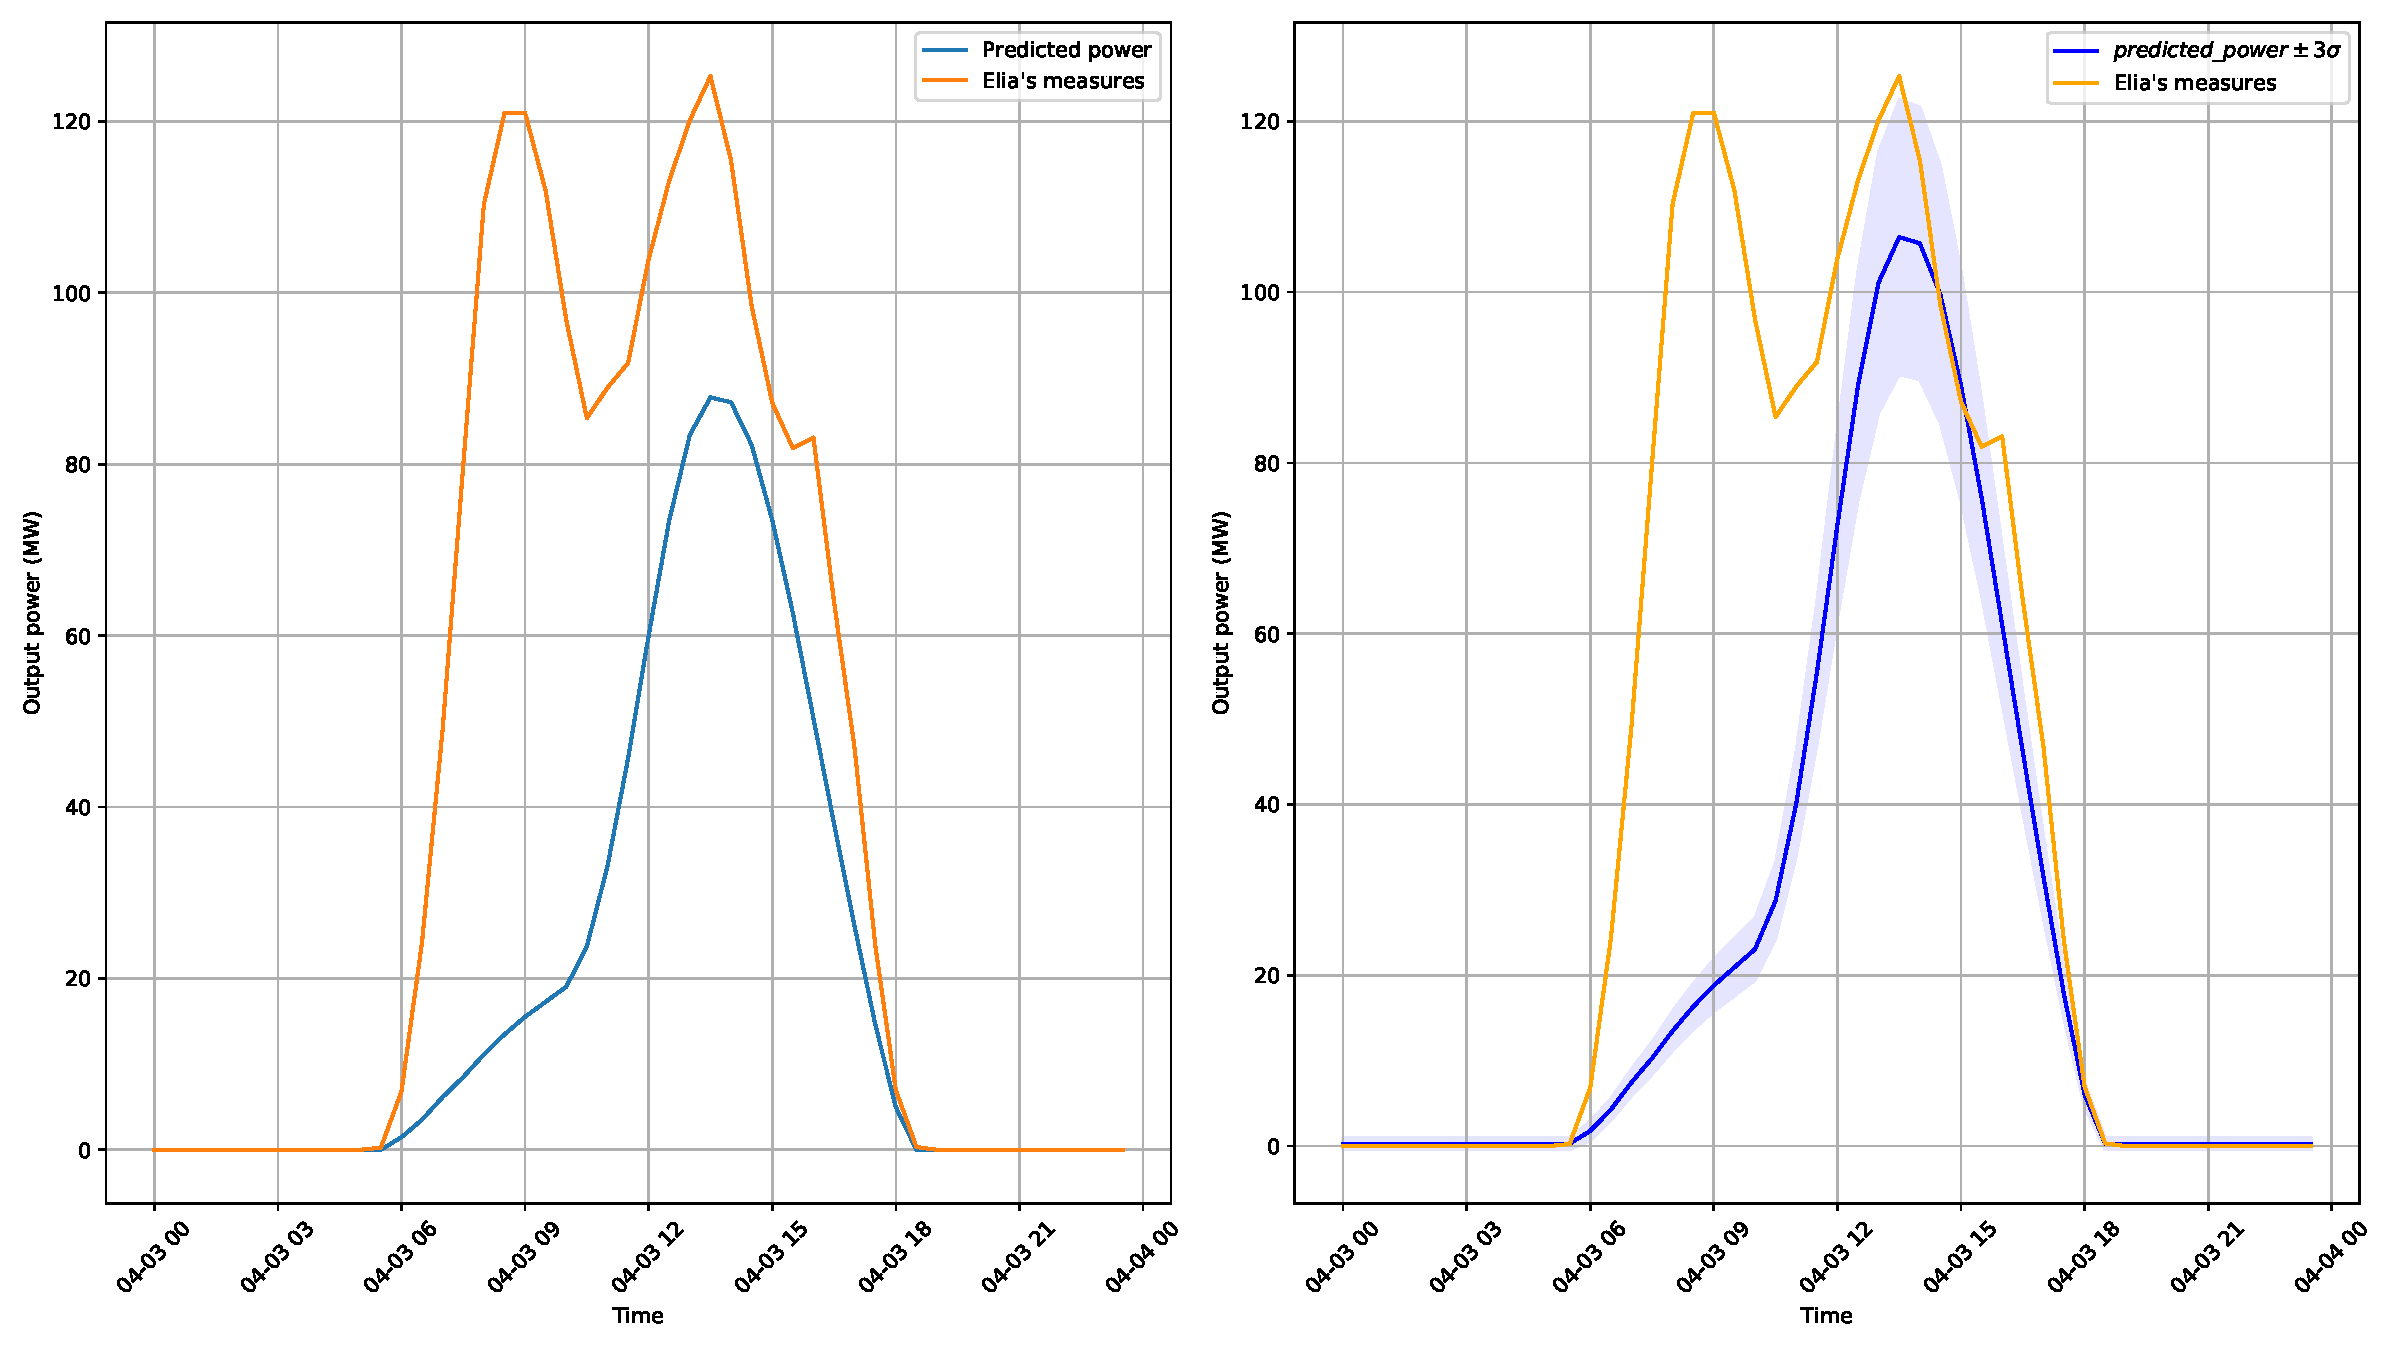
\includegraphics[width=\textwidth]{resources/pdf/comparison_naive_posterior_27-03-2020.pdf}
    \noskipcaption{Comparison between the naive predictive model and the posterior predictive model (April 3rd).}
    \label{fig:naive_posterior_3_april}
\end{figure}
\end{frame}

\begin{frame}{Conclusions}
    \begin{figure}
    \centering
    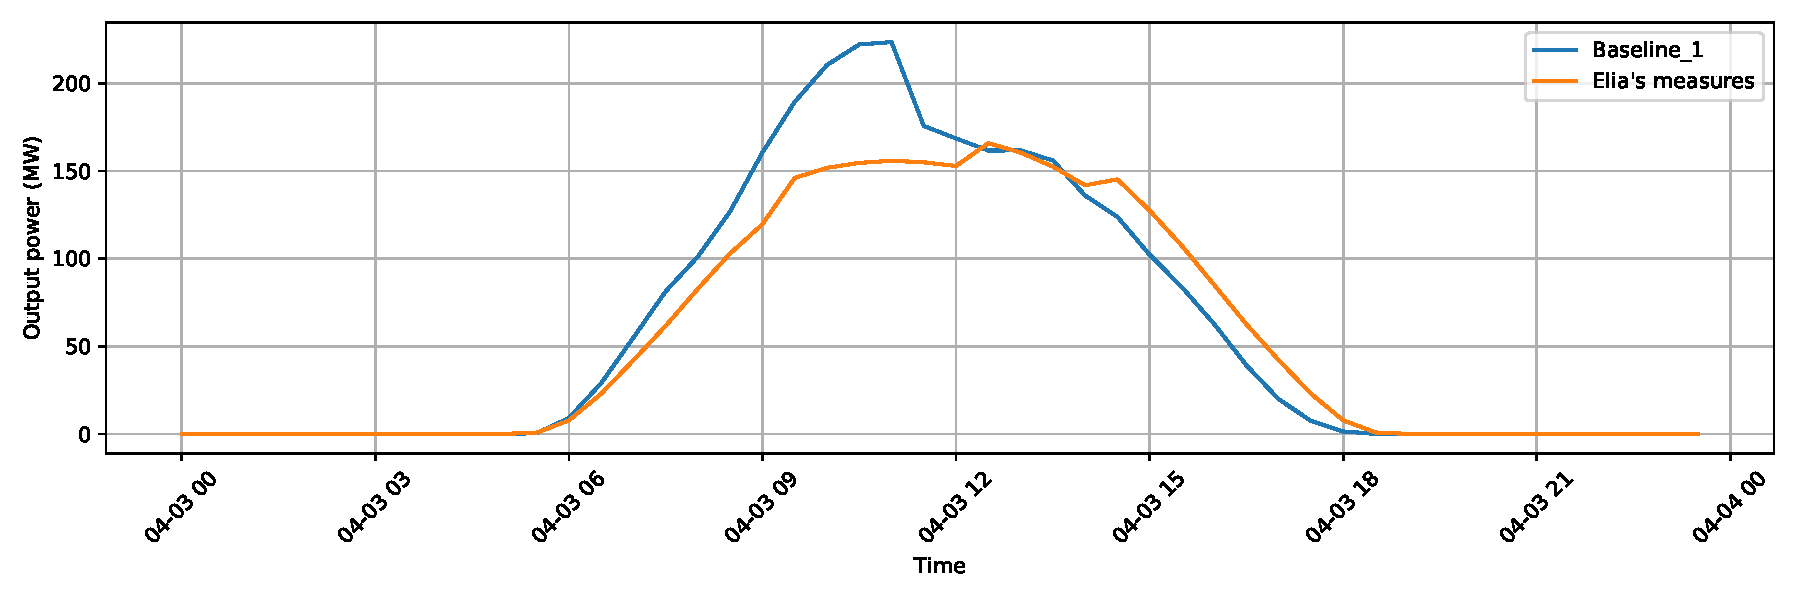
\includegraphics[width=\textwidth]{resources/pdf/baseline_1_27-03-2020.pdf}
    \noskipcaption{Comparison between the first baseline ($D-1$) and Elia's measures (April 3rd).}
    \label{fig:base_1_elia_3_april}
    \end{figure}
\end{frame}

\begin{frame}{Conclusions}
    \begin{figure}
    \centering
    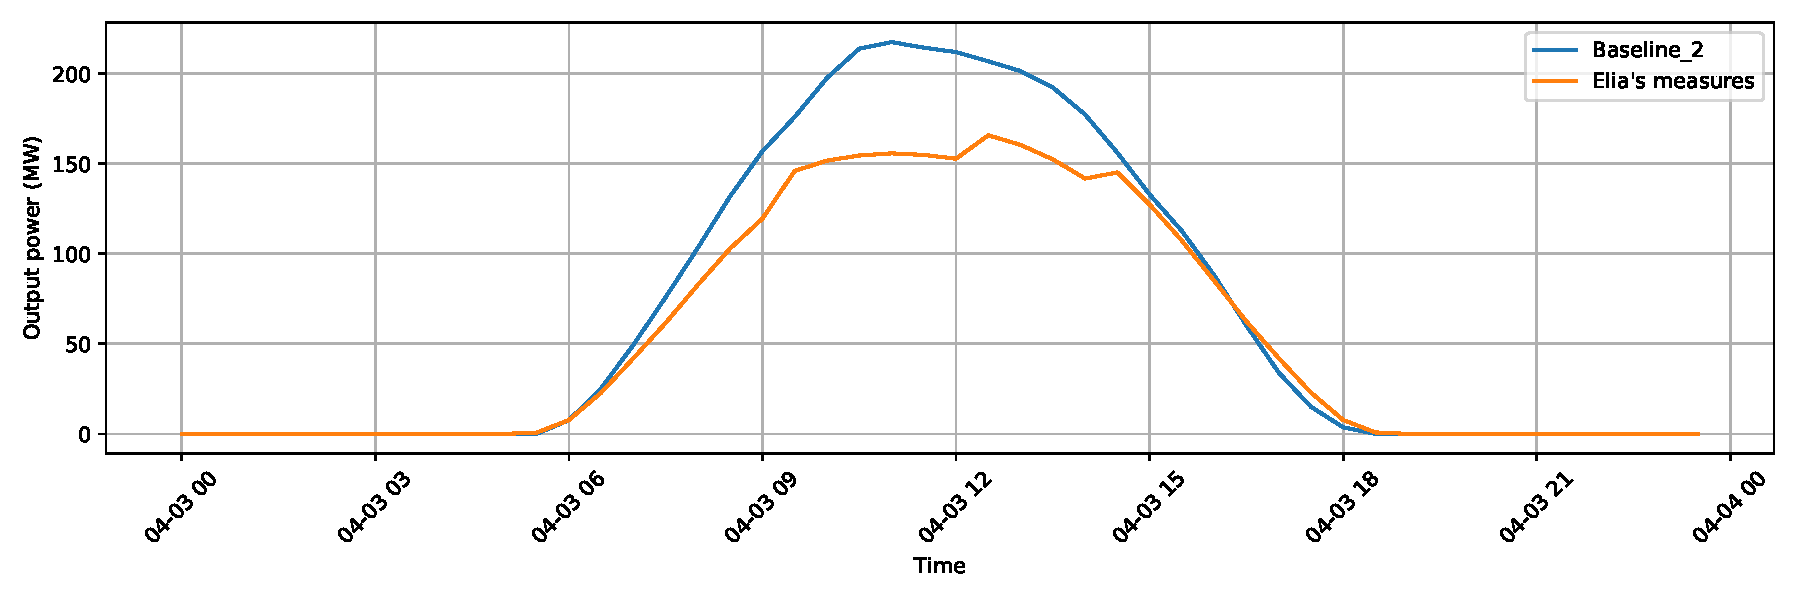
\includegraphics[width=\textwidth]{resources/pdf/baseline_2_27-03-2020.pdf}
    \noskipcaption{Comparison between the second baseline (average) and Elia's measures (April 3rd).}
    \label{fig:base_2_elia_3_april}
    \end{figure}
\end{frame}

\section{Combining panel enumeration and solar model}
\begin{frame}{Outputs of the panel enumerator}
    We managed to get, as outputs:
    \begin{itemize}
        \item The \alert{coordinates} of each panel installation
        \item The \alert{area} of each installation
        \item The \alert{surface azimuth} of each installation
    \end{itemize}
\end{frame}

\begin{frame}{Predicting at the city scale}
    We have managed to process all satellite images for the \alert{city} of Liège and estimated the output production for the \alert{same period} as the previous section. 
\end{frame}

\begin{frame}{Predicting at the city scale}
    \begin{figure}
    \centering
    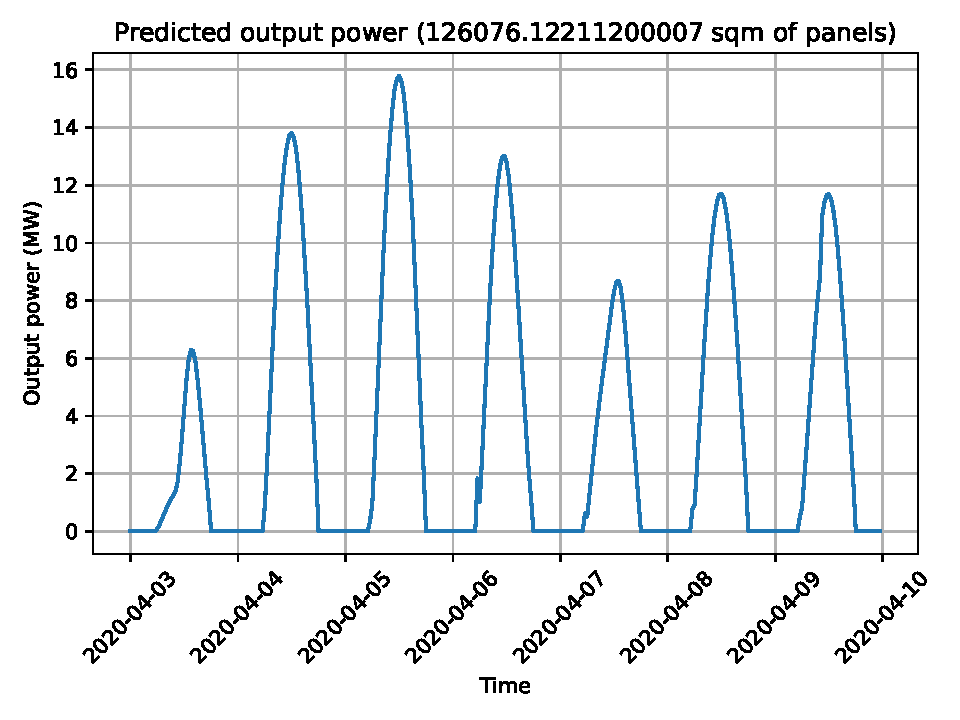
\includegraphics[width=0.65\textwidth]{resources/pdf/solar_liege.pdf}
    \noskipcaption{Predicted production in the city of Liège (using irradiance forecasts).}
    \label{fig:solar_liege}
    \end{figure}
\end{frame}

\begin{frame}{Predicting at the city scale}
    \begin{itemize}
        \item Production \alert{curves} will mainly depend on the irradiance \alert{forecasts'} curve
        \item Order of \alert{magnitude} will depend on the estimated \alert{surface} of panels 
    \end{itemize}
    
    For the city of Liège, we cannot draw conclusions from Elia since they measure \alert{provincial} production.
\end{frame}

\section{Next objectives}
\begin{frame}{Next objectives}
    \begin{itemize}
        \item Conduct the abovedefined tests on a \alert{larger} period of April, using irradiance \alert{forecasts}
        \item Try and get \alert{reliable} estimates of the panel installations in the \alert{province} of Liège, to compare with Elia's measurements
    \end{itemize}
\end{frame}

\section{Photovoltaic panels enumeration}

\begin{frame}{Reminder}
    Two objectives :
    
    \begin{enumerate}
        \item Apply our model to our \alert{initial problem}, \emph{i.e.} the enumeration of photovoltaic panels in the province of Liège.
        \item Evaluate more precisely the precision of our model (\alert{U-Net}) using the \alert{average precision} metric.
    \end{enumerate}
\end{frame}

\begin{frame}{WalOnMap}
    \alert{WalOnMap} \cite{walonmap} images are organized under the \alert{Web Map Tiles Service} standard \cite{maso2010opengis}.
    
    We used the \texttt{owslib} package to request the tiles (the images) \alert{one by one}.
    
    To save space and ease the following computations, the produced masks were saved as polygons unde the \alert{VGG Image Annotator} \cite{dutta2019via} format.
\end{frame}

\begin{frame}[standout]
    VGG Image Annotator
\end{frame}

\begin{frame}{Enumeration}
    We ran into two major issues before succeeding to apply the model.
    
    \begin{itemize}
        \item \alert{WalOnMap} images are much more \alert{blurry} than the one of \alert{California}. Therefore, we added further data augmentation transformations like blurring, smoothing and sharpening.
        \item The scales of the two datasets are dissimilar. One pixel in Wallonia is \alert{\SI{0.14}{\meter}} and one pixel in California is \alert{\SI{0.30}{\meter}}. We decided to upscale the Californian images by a factor of two.
    \end{itemize}
\end{frame}

\begin{frame}{Enumeration}
    If \alert{most panels} were detected, a lot of \alert{shadows} and \alert{dark roofs} were also.
    
    To evaluate the actual performances of the model, we \alert{annotated by hand} (using \alert{VIA}) more than \alert{600} images.
\end{frame}

\begin{frame}{Enumeration}
    \begin{figure}
        \centering
        \vspace{-0.5em}
        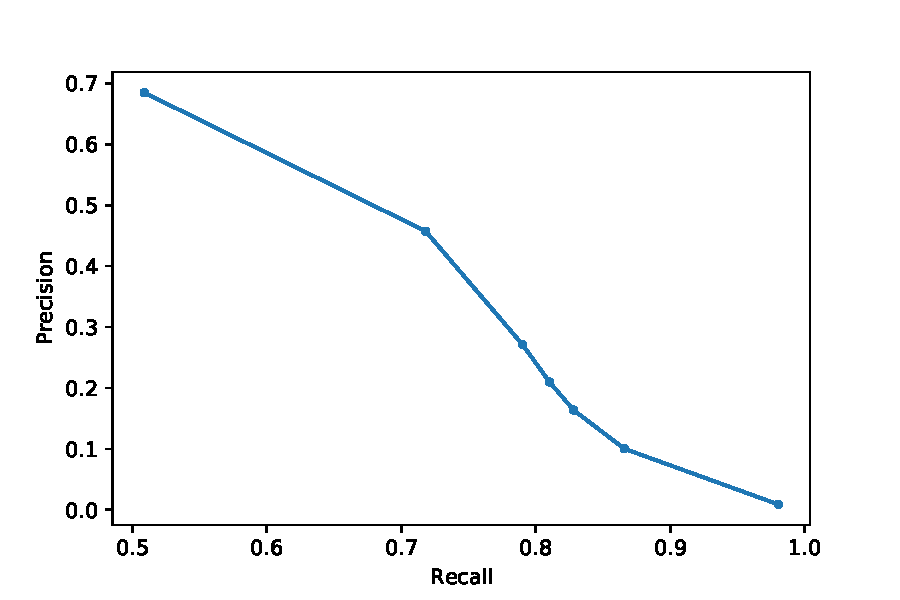
\includegraphics[width=0.95\textwidth]{resources/pdf/precision_recall_before.pdf}
        \caption{Precision-Recall curve of U-Net before fine tuning.}
    \end{figure}
\end{frame}

\begin{frame}{Enumeration - Fine tuning}
    We \alert{fine tuned} our model for \alert{20} more epochs on a subset of our hand-annotated images.
\end{frame}

\begin{frame}{Enumeration - Fine tuning}
    \begin{figure}
        \centering
        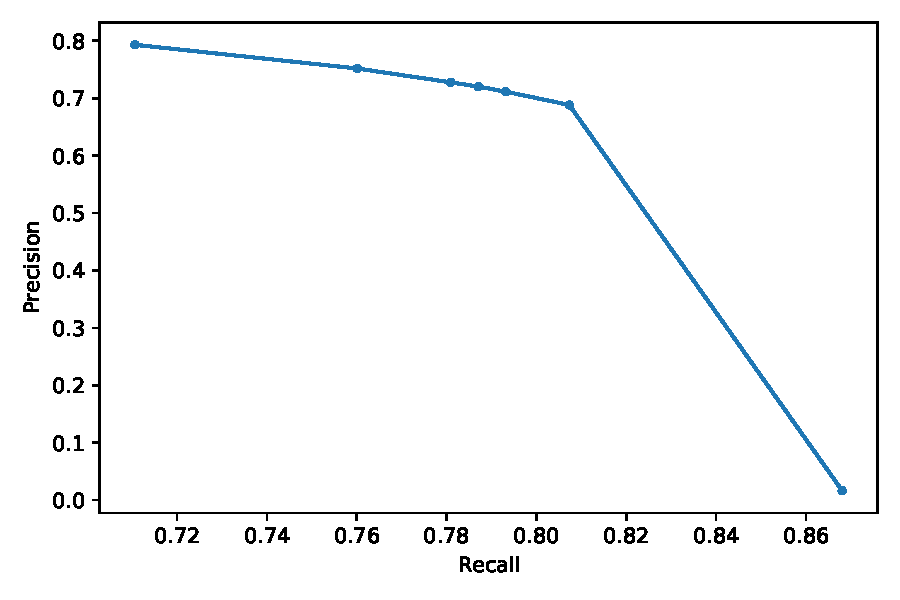
\includegraphics[width=0.95\textwidth]{resources/pdf/precision_recall_after.pdf}
        \caption{Precision-Recall curve of U-Net after fine tuning.}
    \end{figure}
\end{frame}

\begin{frame}[standout]
    Quick demonstration
\end{frame}

\begin{frame}{Enumeration - Binding}
    There was still to bind our enumeration model with the \alert{photovoltaic production model}.
    
    Since we stored polygons (cf. VIA format) and the tiles are geo-referenced, it was not too hard to compute the \alert{localization} and \alert{area} of each installation we had detected.
    
    The \alert{azimuth} is deduced from the \alert{minimal area bounding rectangle} of the polygon.
\end{frame}

\begin{frame}{Average precision}
    \begin{figure}
        \centering
        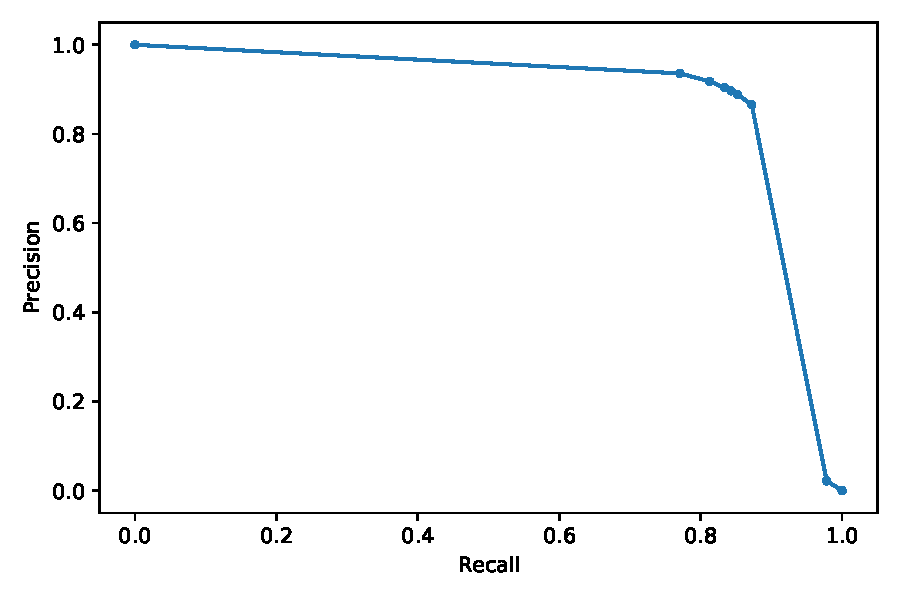
\includegraphics[width=0.9\textwidth]{resources/pdf/precision_recall.pdf}
        \caption{Precision-Recall curve of U-Net on the Californian validation set.}
    \end{figure}
\end{frame}

\begin{frame}{Average precision}
    The average precision is \alert{\SI{88.6}{\percent}}.
\end{frame}

\section{Wind power production}

\begin{frame}{Addition of new variables}
    The first idea was to add the following variables:
    \begin{itemize}
        \item Total power monitored by Elia
        \item Yearly total installed power in Wallonia
        \item One day before power measurements
    \end{itemize}
\end{frame}

\begin{frame}{Addition of new variables}
    \begin{center}
        \resizebox{\textwidth}{!}{
            \begin{tabular}{|c|c|c|c|c|c|}
                \hline
                Protocol 2 & Method & MAE\footnotemark[1] & sMAE\footnotemark[1] & MQL10\footnotemark[1] & MQL90\footnotemark[1] \\ \hline
                \multirow{2}{*}{\alert{With the new variables}} & Extra Trees & 28.27 & 4.43\% & 53.42 & 56.33 \\ \cline{2-6}
                 & Gradient Boosting & 30.98 & 4.27\% & 51.23 & 55.21 \\ \hline
                \multirow{2}{*}{Without the new variables} & Extra Trees & 28.13 & 4.03\% & 46.63 & 50.32 \\ \cline{2-6}
                 & Gradient Boosting & 31.11 & 4.46\% & 48.32 & 47.91 \\ \hline
            \end{tabular}
        }
    \end{center}
    \footnotetext[1]{\SI{}{\mega \watt}}
\end{frame}

\begin{frame}{Multilayer Perceptron}
    A new type of supervised learning has been tested: the MLP.
    \begin{center}
        \begin{tabular}{|c|c|c|}
            \hline 
            Method & MAE\footnotemark[1] & sMAE\footnotemark[1] \\ \hline
            \alert{MLP with new variables} & 30.98 & 4.27\%  \\ \hline
            Gradient Boosting with new variables & 30.98 & 4.27\% \\ \hline
            Gradient Boosting without new variables & 31.11 & 4.46\% \\ \hline
        \end{tabular}
    \end{center}
    \footnotetext[1]{\SI{}{\mega \watt}}
\end{frame}

\begin{frame}{Conclusion}
    \begin{itemize}
        \item Adding new temporal variable has not helped
        \item All considered supervised learning method seemed to cap at a threshold around \SI{30}{\mega \watt} in terms of MAE.
    \end{itemize}
    However,
    \begin{itemize}
        \item The set of variable that explains the output can be made more refined
    \end{itemize}
\end{frame}

\begin{frame}{New learning set}
   \begin{itemize}
       \item Weather measurements only
       \item At every 68 known wind farms of Wallonia (data from 2018-2019)
       \item Each weather measurement is 7-dimensional (wind speed, wind gust, wind bearing, humidity, temperature, air density, pressure
       \item In total, 476 weather variables
       \item Around two years of yearly measurements, resulting in \num{18 000} samples.
   \end{itemize}
\end{frame}

\begin{frame}{New learning set}
    \begin{figure}[H]
        \centering
        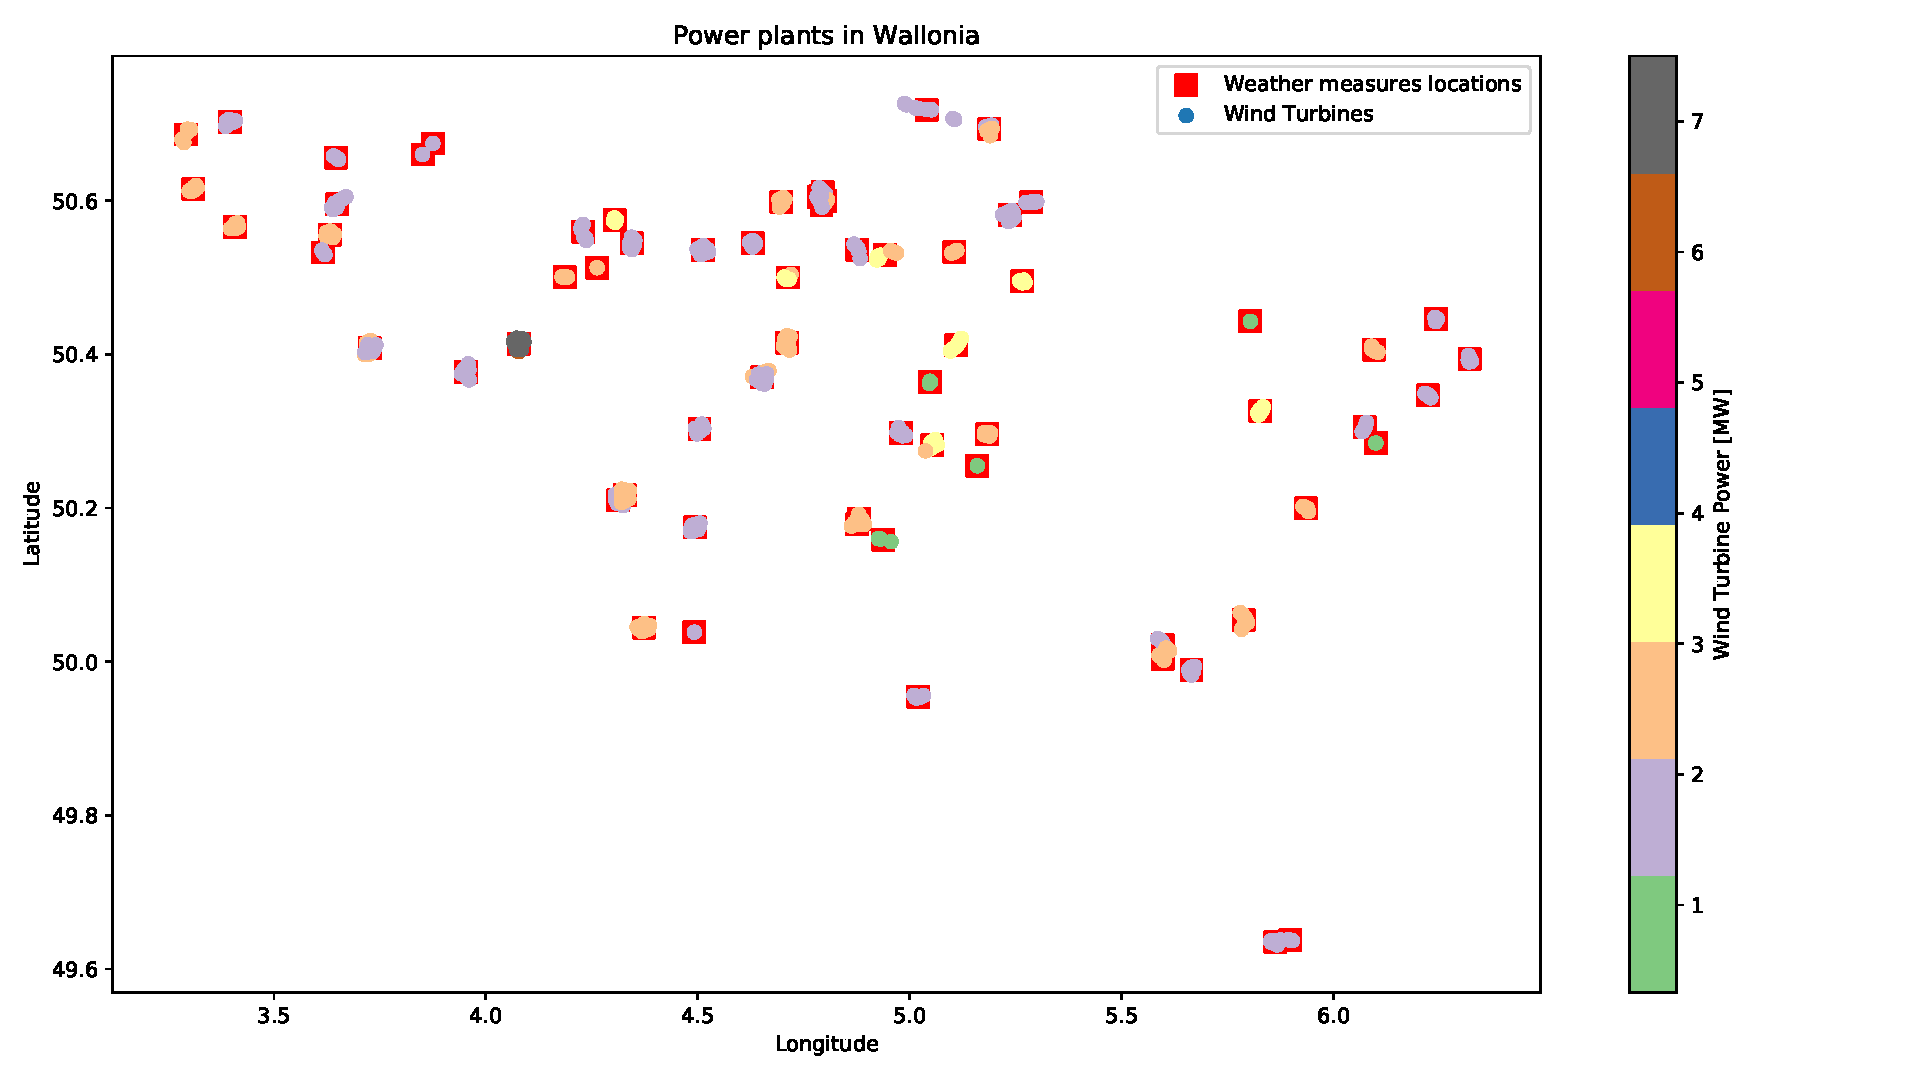
\includegraphics[width=\textwidth]{resources/pdf/power_plants.pdf}
        \caption{Wind turbines and weather measurements}
        \label{fig:wt_wallonia}
    \end{figure}
\end{frame}

\begin{frame}{Results on validation set}
    \begin{tabular}{|c|c|c|c|c|}
        \hline
        Method & MAE\footnotemark[1] & sMAE\footnotemark[1] & MQL10\footnotemark[1] & MSL90\footnotemark[1] \\ \hline
        Gradient Boosting 15 & 31.11 & 4.46\% & 48.32 & 47.91 \\ \hline
        Gradient Boosting 68 & 28.46 & 3.92\% & 51.19 & 49.33 \\ \hline
    \end{tabular}
    \footnotetext[1]{\SI{}{\mega \watt}}
\end{frame}

\begin{frame}{Results on test set}
    The test set is composed of day-ahead numerical weather prediction (DANWP) instead of weather measurements. Only 9.5 days have been collected for now.
    \begin{center}
    \begin{tabular}{|c|c|c|}
        \hline
        Model & Validation MAE [\SI{}{\mega \watt}] & Test MAE [\SI{}{\mega \watt}] \\ \hline
        15-measurements & 31.1 & 45.42 \\ \hline
        68-measurements & 28.46 & 40.72 \\ \hline
    \end{tabular}
    \end{center}
\end{frame}

\begin{frame}{Results on test set}
    \begin{figure}[H]
        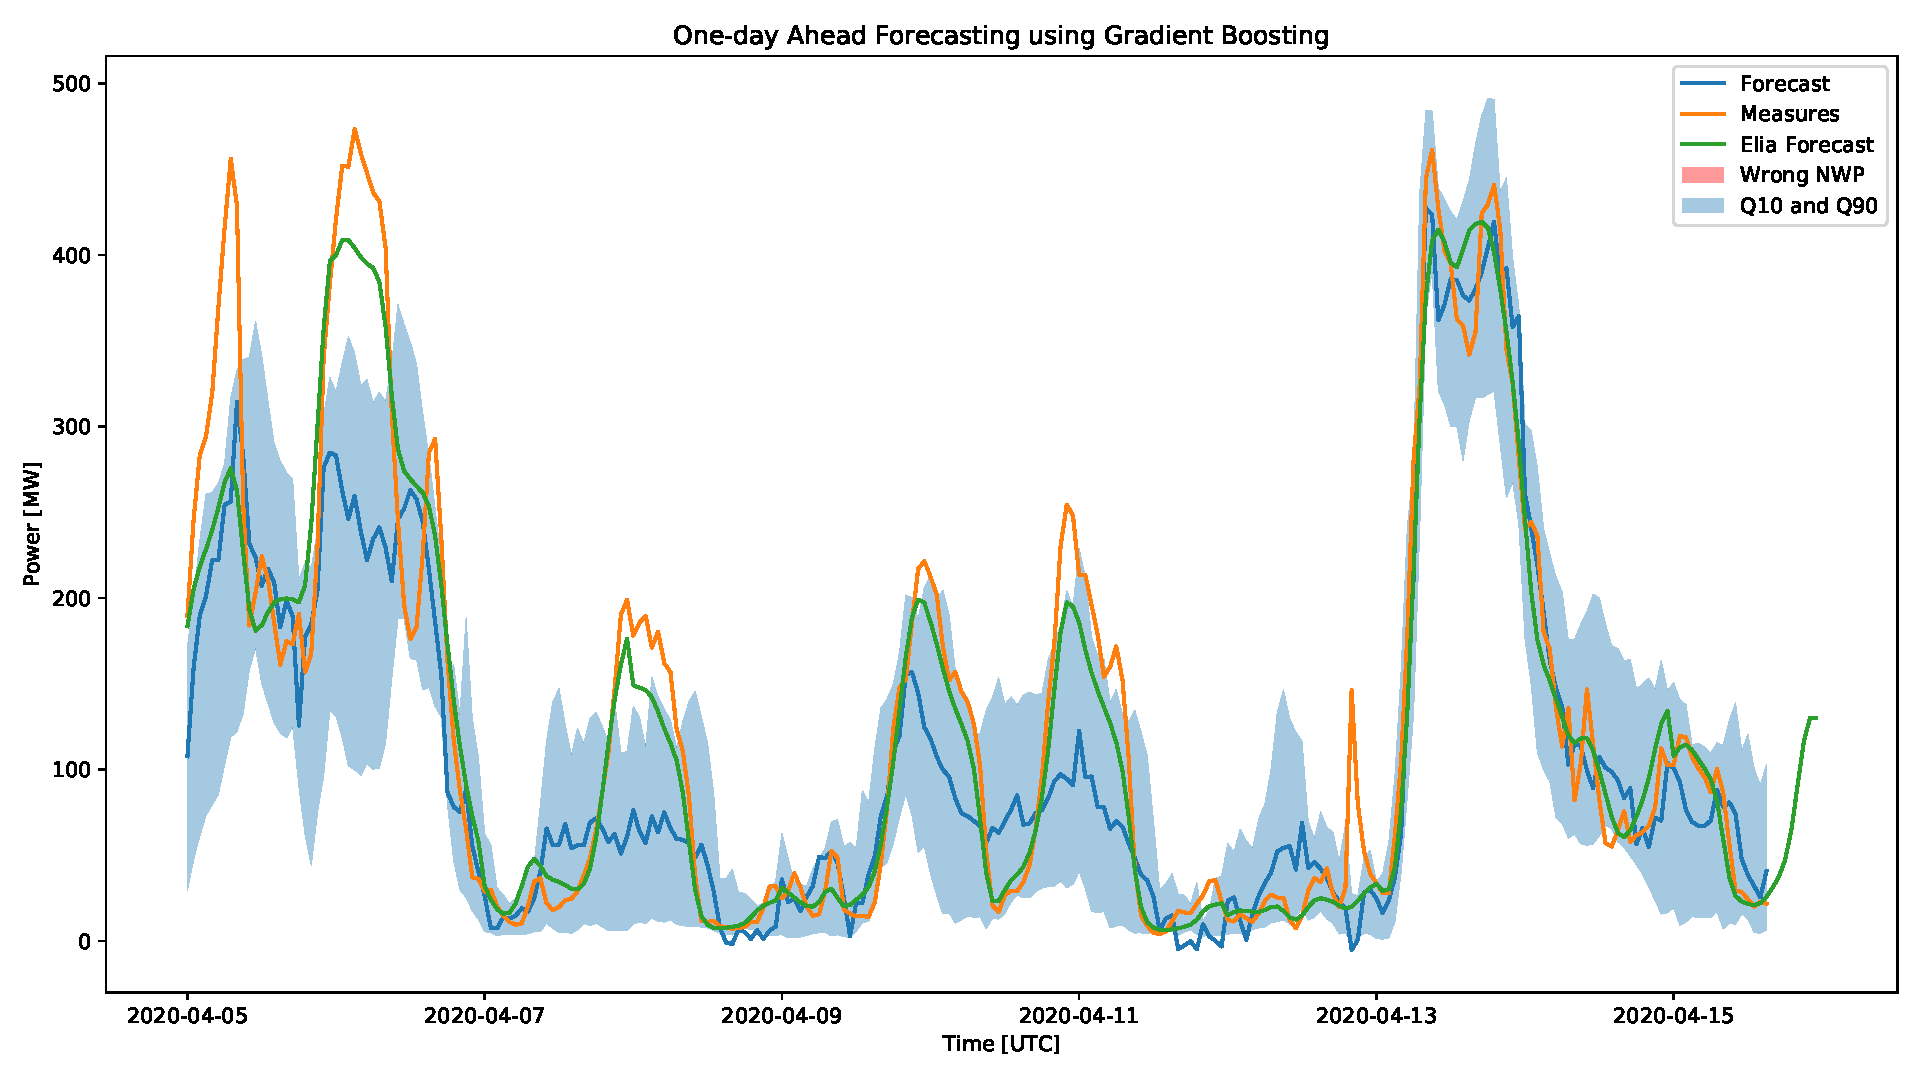
\includegraphics[width=\textwidth]{resources/pdf/odaf15_april.pdf}
        \caption{15-measurements Gradient Boosting}
    \end{figure}
\end{frame}

\begin{frame}{Results on test set}
    \begin{figure}[H]
        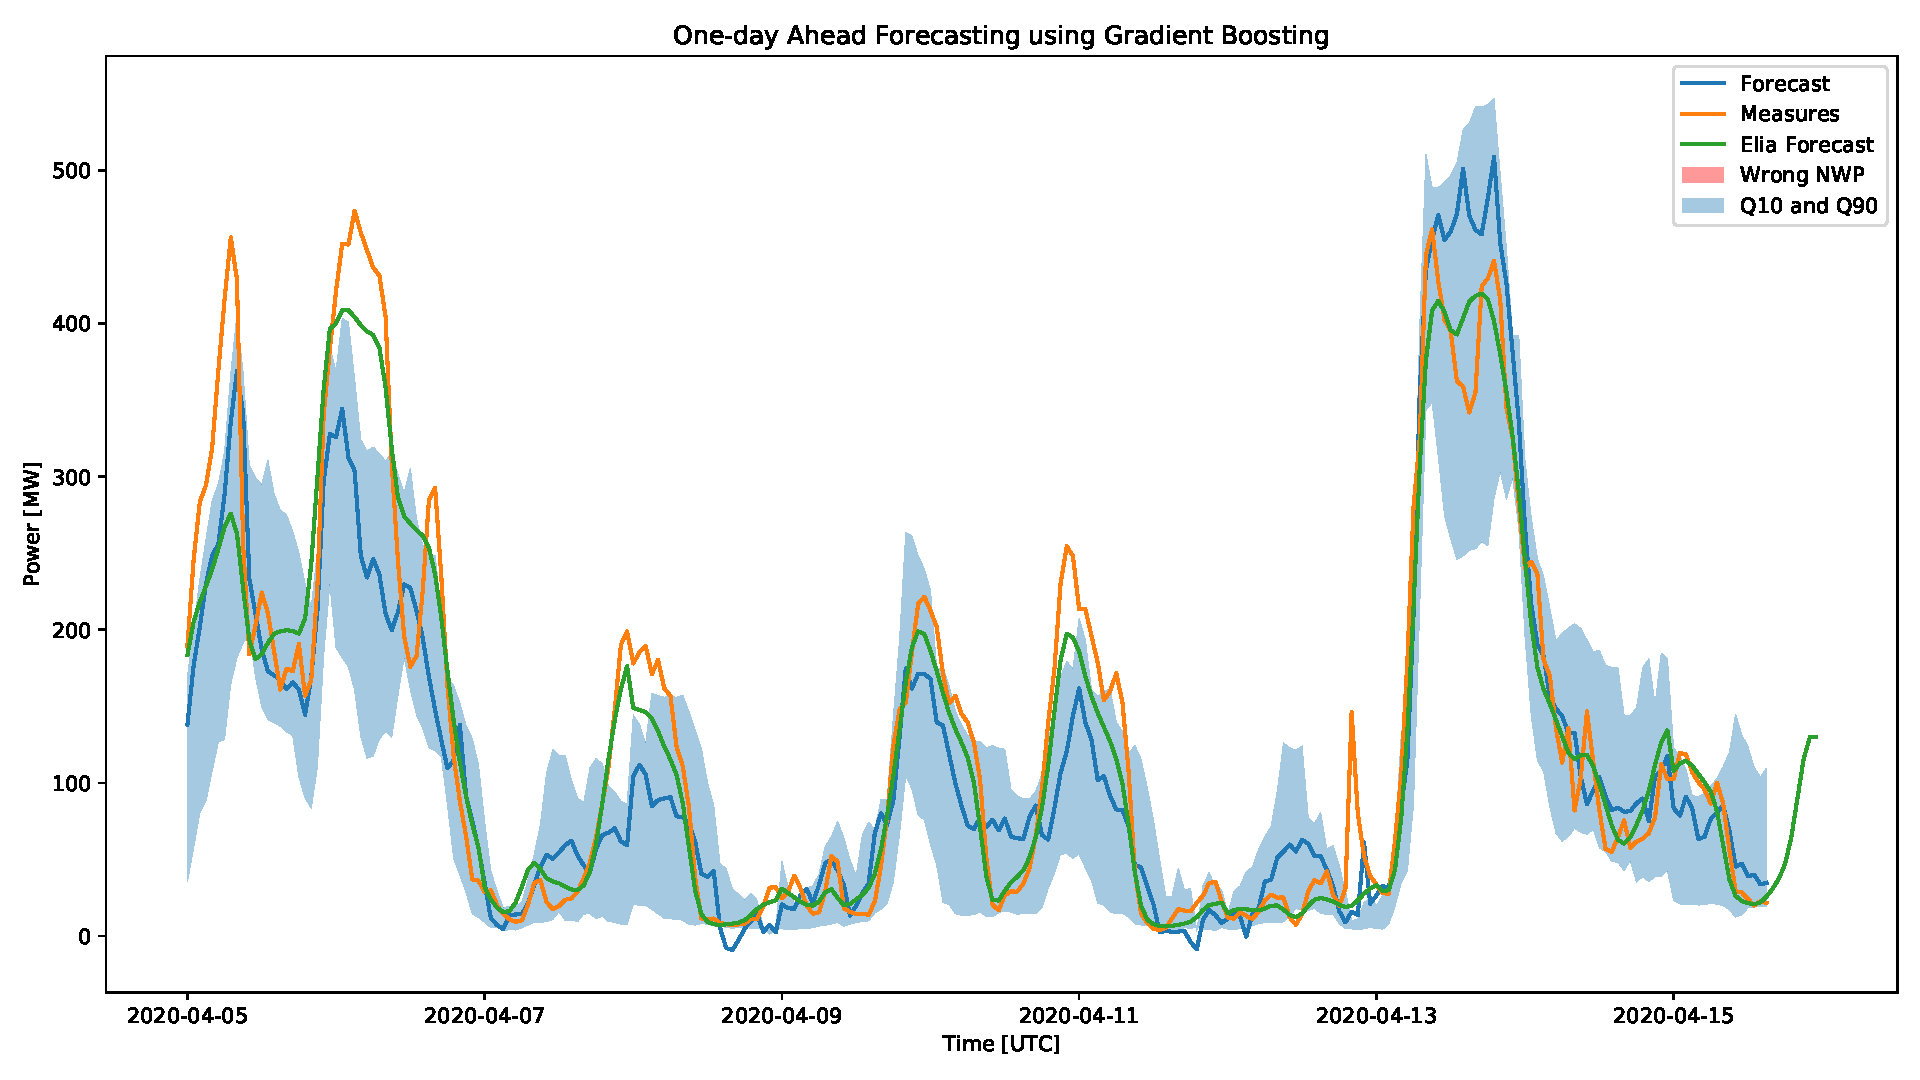
\includegraphics[width=\textwidth]{resources/pdf/odaf68_april.pdf}
        \caption{68-measurements Gradient Boosting}
    \end{figure}
\end{frame}

\begin{frame}{Features importances}
    \begin{figure}[H]
        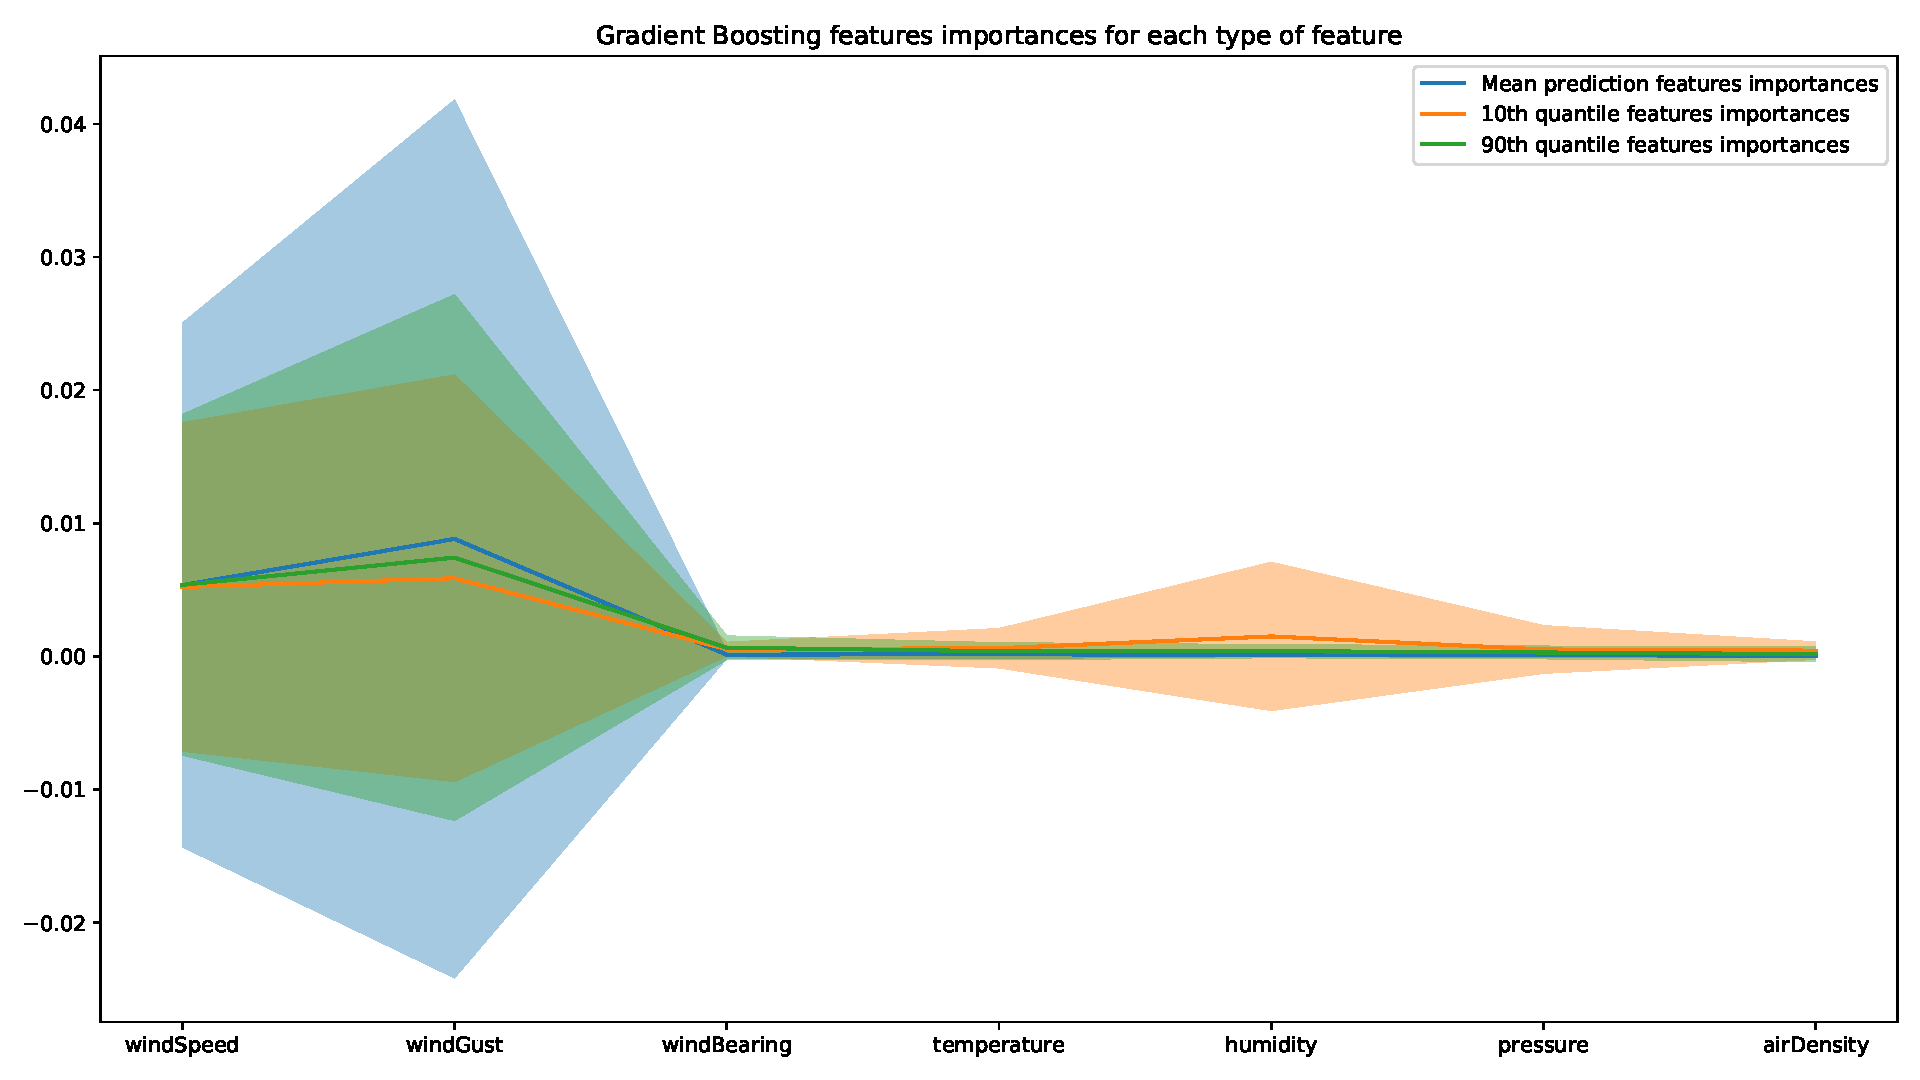
\includegraphics[width=\textwidth]{resources/pdf/fi.pdf}
        \caption{Features Importance}
    \end{figure}
\end{frame}

\begin{frame}{Results on test set on 13.5 days}
    The MAE was 40.72 MW on the 9.5-days test set, and is 36.89 MW on the 13.5-days test set.
    \begin{figure}[H]
        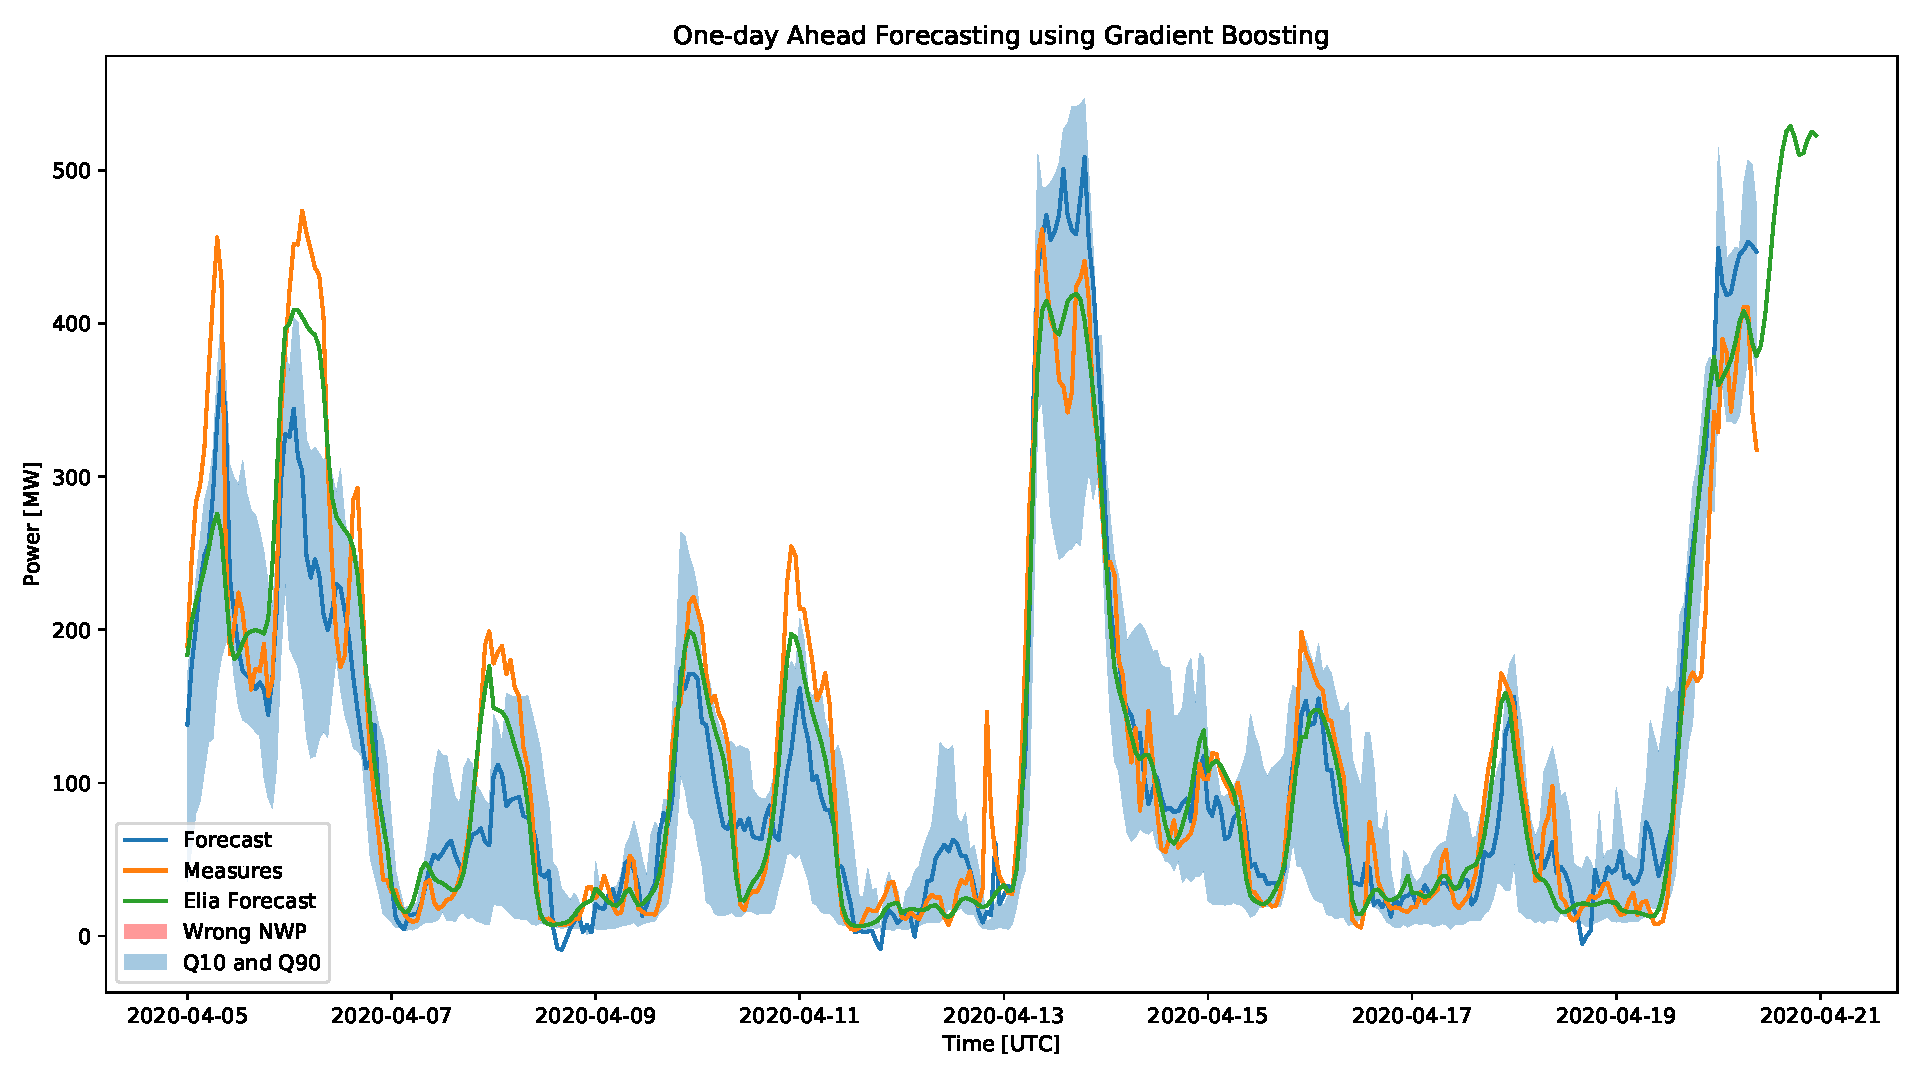
\includegraphics[width=\textwidth]{resources/pdf/forecast.pdf}
    \end{figure}
\end{frame}

\begin{frame}[allowframebreaks]
    \printbibliography
\end{frame}

\end{document}
